\documentclass[]{report}
\usepackage[hmargin=1.25in,vmargin=1in]{geometry} %调整页边距
% \usepackage[inner=1in,outer=1.25in]{geometry} %书籍左右不等宽排版
\usepackage[utf8]{inputenc}
\usepackage[]{ctex} %据说可以直接调用诸如 \kaishu \fangsong \heiti 的命令修改字体
\usepackage[svgnames]{xcolor} % Using colors
% \usepackage{background} % To include background images
\usepackage{fancyhdr} % Needed to define custom headers/footers
\usepackage[]{xeCJK}
\setCJKmainfont[BoldFont = STHeiti, ItalicFont = STKaiti]{Songti SC Light} %中文主字体
\setCJKsansfont[BoldFont = Weibei SC, ItalicFont = HanziPen SC]{Xingkai SC Light} %中文无衬线字体
\setCJKmonofont[BoldFont = Libian SC, ItalicFont = STFangsong]{Yuanti SC Light} %中文等宽字体
\setmainfont{Times New Roman} %\rmfamily
\setsansfont[ItalicFont = American Typewriter]{Comic Sans MS} %\sffamily
\setmonofont{Courier} %\ttfamily
\newfontfamily\monaco{Courier} % 用于代码段字体设置
\newfontfamily\OldCaption{Bodoni 72 Smallcaps Book} %用于全大写字母的标题
\usepackage{titlesec}
% 一下为适用于笔记/整理的板式(第几章-第几节)
% \titleformat{\chapter}{\centering\huge\bfseries}{第~\thechapter~章}{1em}{}
% \titleformat{\section}{\Large\bfseries}{第~\thesection~节}{1em}{}
% 一下为适用于作业的板式(第几次-第几题-abcd问)
\titleformat{\chapter}{\centering\huge\bfseries}{第六次作业}{1em}{}
\titleformat{\section}{\Large\bfseries}{第~\thesection~题}{1em}{}
\renewcommand{\thesubsection}{(\alph{subsection})}
\usepackage{lipsum} %填充文本

\usepackage{ulem} %解决下划线、删除线之类的
\usepackage{listings}
\lstset{
language=C++,
numberstyle = \monaco,
basicstyle = \monaco,
keywordstyle = \color{blue}\bfseries,
commentstyle=\color[HTML]{006400},
tabsize = 4,
%backgroundcolor=\color{bg}
emph = {int,float,double,char},emphstyle=\color{cyan},
emph = {[2]const, typedef},emphstyle = {[2]\color{red}} }

\makeatletter
\newif\if@restonecol
\makeatother
\let\algorithm\relax
\let\endalgorithm\relax
\usepackage[linesnumbered,ruled,vlined]{algorithm2e}%[ruled,vlined]{
\usepackage{algpseudocode}
\usepackage{amsmath}
\renewcommand{\algorithmicrequire}{\textbf{Input:}}  % Use Input in the format of Algorithm
\renewcommand{\algorithmicensure}{\textbf{Output:}} % Use Output in the format of Algorithm

\usepackage{amsmath} %数学公式问题
\usepackage{amsthm} %公式环境,如proof
\usepackage{booktabs} %三线表
\newcommand{\tabincell}[2]{\begin{tabular}{@{}#1@{}}#2\end{tabular}} %解决单元格内部换行的问题
% 比如这个 Beijing & 0,5 & 1,6 & 2,7 & 3,8 & 4,9 & The number changes every 3 months \\
% 改成这个 \tabincell{l}{Beijing}& \tabincell{c}{0,5}& \tabincell{c}{1,6}& \tabincell{c}{2,7}& \tabincell{c}{3,8}& \tabincell{c}{4,9}& \tabincell{c}{The number changes \\ every 3 months} \\
% 一个单元格过长,整行都需要修改
% 可以配合 \resizebox*{h-width}{v-width}{contents, e.g.tabular} 使用

\usepackage{mathrsfs} %在公式里面使用那个最花的字体
\usepackage{amssymb} %公式里面用空心黑体和旧式字体
\usepackage{amssymb} %AMS符号
\usepackage{amsthm} %AMS定理环境

\usepackage{markdown} %使用markdown语法,在编译时需要打开 shell-escape 标记,即 $ xelatex --shell-escape example.tex
\markdownSetup{hashEnumerators = true} %允许使用 #. 的方式编写有序列表
\markdownSetup{inlineFootnotes = true} %允许使用脚注形式的超链接,调用语法为 [anchor](uri), ^[footnote], <uri>
\markdownSetup{fencedCode = true} %以反引号和缩进来插入代码段,相当于 verbatim
\markdownSetup{
  pipeTables = true
} %支持表格的用法 (图片已经在markdown包里面支持了)
% \usepackage{booktabs} %解决三线表的线条粗细问题

\usepackage{graphicx} %插入图片
\usepackage{pdfpages} %插入PDF文件
\usepackage{makeidx}

\usepackage{tikz} %带圈字符
\usepackage{etoolbox} %带圈字符 (提供robustify)
\usepackage{enumitem}
\newcommand*{\circled}[1]{\lower.7ex\hbox{\tikz\draw (0pt, 0pt)%
    circle (.5em) node {\makebox[1em][c]{\small #1}};}} %新定义命令:带圈字符
\robustify{\circled}
% \usepackage{enumerate} %有序列表

\usepackage{hyperref} %超链接
% \usepackage[hidelinks]{hyperref} %隐藏超链接的红框
\markdownSetup{
  inlineFootnotes = true,
  renderers = {
    link = {\href{#3}{#1}},
  }
} % markdown块中使用直接点进去的超链接
% \setlist[enumerate,1]{label=(\arabic*).,font=\textup,leftmargin=7mm,labelsep=1.5mm,topsep=0mm,itemsep=-0.8mm}
% \setlist[enumerate,2]{label=(\alph*).,font=\textup,leftmargin=7mm,labelsep=1.5mm,topsep=-0.8mm,itemsep=-0.8mm}

\usepackage{braket}

%%%%%% Setting up the style

% \setlength\parindent{0pt} % Gets rid of all indentation
% \backgroundsetup{contents={\includegraphics[width=\textwidth]{ustc-name.pdf}},scale=0.4,placement=top,opacity=0.6,color=cyan,vshift=-20pt} %  USTC Logo

\pagestyle{fancy} % Enables the custom headers/footers

% 使用默认的Chapter页眉
% \lhead{} \rhead{} % Headers - all  empty

% \title{\vspace{-1.8cm}  \color{DarkRed} Laboratory Rotation Report}
% \subtitle{Title of the proposal % Title of the rotation project
% \vspace{-2cm} }
% \date{\today} % No date

\lfoot{\color{Grey} \textit{艾语晨}}  % Write your name here
\rfoot{ \color{Grey} 算法作业 }
\cfoot{\color{Grey} \thepage}

\renewcommand{\headrulewidth}{0.0pt} % No header rule
\renewcommand{\footrulewidth}{0.4pt} % Thin footer rule

\title{算法基础第六次作业}
\author{艾语晨~PB18000227}
\date{\today}

\linespread{1.3} %行间距为1.3倍默认间距 (1.3 x 1.2倍字符宽度)

\makeindex

\begin{document}
\theoremstyle{definition} \newtheorem{theorem}{Thm}[section] %定义一个定理Thm,序号为section的下一级序号
\theoremstyle{definition} \newtheorem{definition}{Def}[section] %定义一个定义Def,序号为section的下一级序号
\theoremstyle{plain} \newtheorem{lemma}{lemma}[section] %引理

	\maketitle
	\newpage

	\tableofcontents
	\newpage

	\chapter{}
	\section{钢条切割}
	由题可知,最优切割收益公式为:
	\[r_n=\max\{p_n,\max_{1\le i\le n-1}\{r_i+r_{n-i}-c\}\}\]
	算法MEMOIZED-CUT-ROD-AUX修改为如下:
	\begin{algorithm}
		\caption{MEMOIZED-CUT-ROD-AUX(p,n,r)}
		\If{$r[n]\ge0$}{
			\Return{r[n]}
		}
		\If{$n==0$}{
			$q=0$
		}
		\Else{
			$q=-\infty$\\
			\For{$i=1$ $\mathbf{to}$ $n$}{
				$q=\max(q,p[i]+MEMOIZED-CUT-ROD-AUX(p,n-i,r))$
			}
		}
		$r[n]=q$\\
		\Return{q}
	\end{algorithm}
	\section{有向无环图中的最长简单路径}
	设$s'$为一个与$s$相邻的顶点,则有如下递推式:
	\[LONGEST(G,s,t) = 1 + max_{s\sim s'}{LONGEST(\{G-V\},s′,t)}\]\par
	其中{G-V}表示图G去掉顶点V和与V相连的所有边之后的子图\par
	\section{最优二叉搜索树}
	最优二叉搜索树如下图所示:
	\begin{figure}
		\centering
		\begin{minipage}{40em}
			\centering
			
\includegraphics[scale = 0.4]{images/3_Optimal_BST.png}
			\caption{最优二叉搜索树}
		\end{minipage}
	\end{figure}\par
	其代价为:
	\begin{figure}
		\centering
		\begin{minipage}{20em}
			\centering
			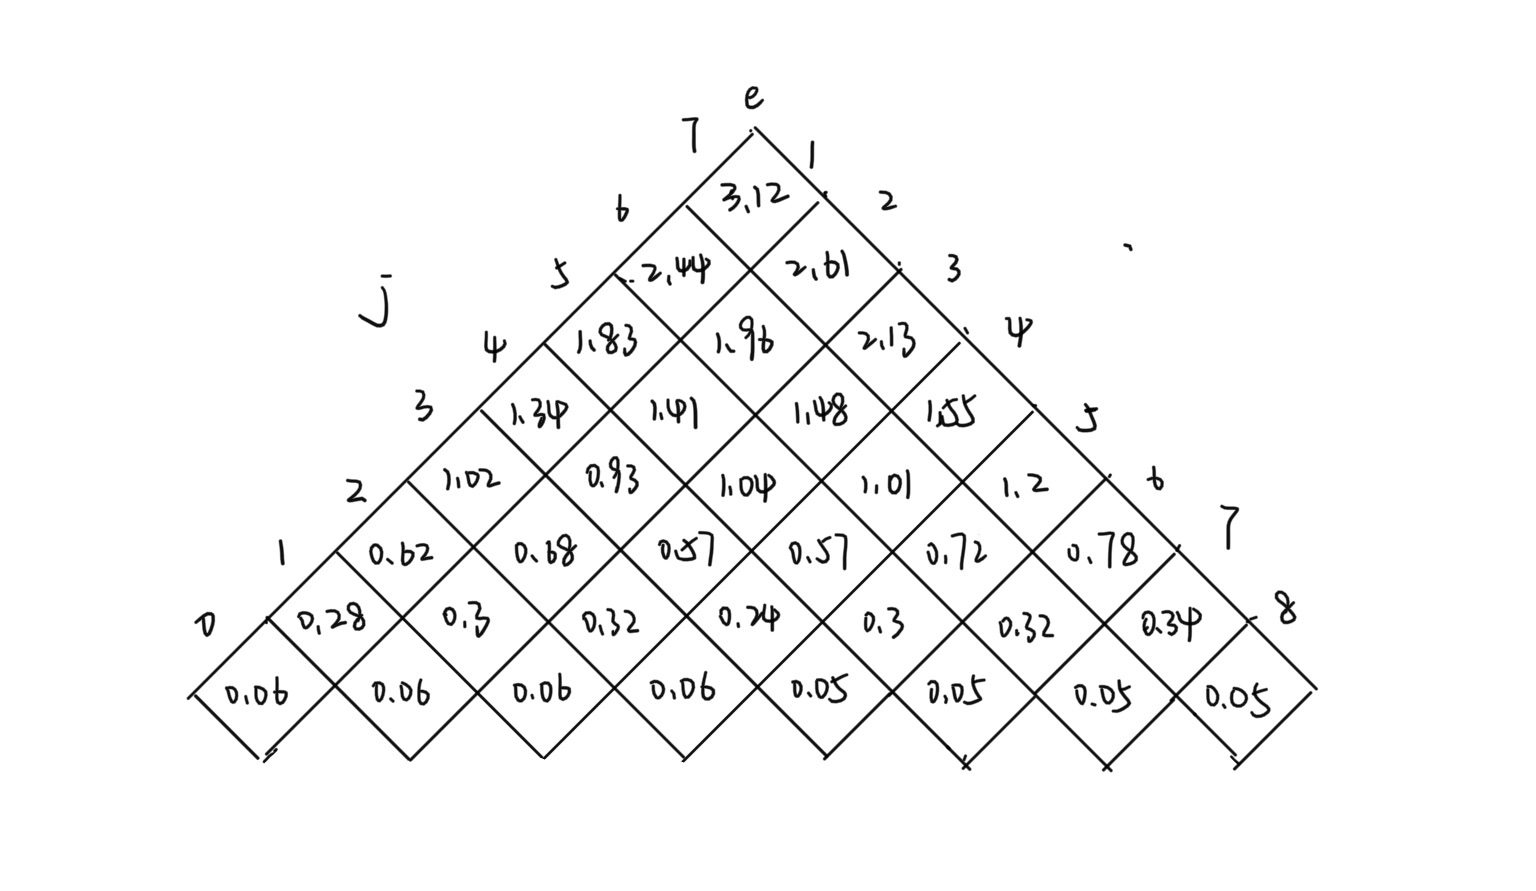
\includegraphics[scale = 0.13]{images/3_2.png}
		\end{minipage}
		\begin{minipage}{20em}
			\centering
			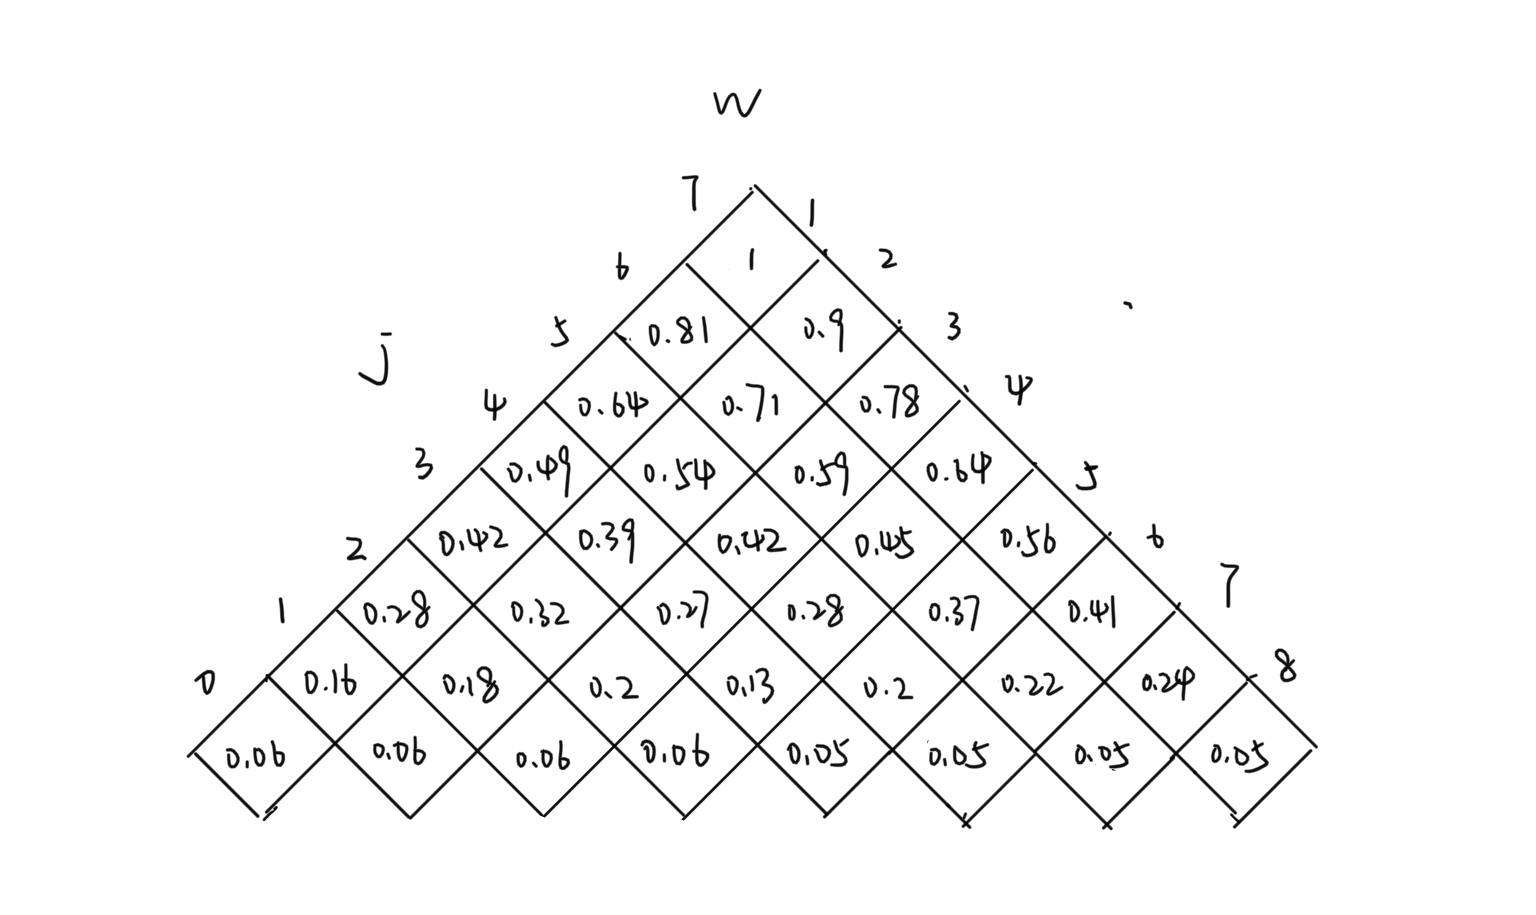
\includegraphics[scale = 0.13]{images/3_3.png}
		\end{minipage}
	\end{figure}
	\begin{figure}
		\centering
		\begin{minipage}{40em}
			\centering
			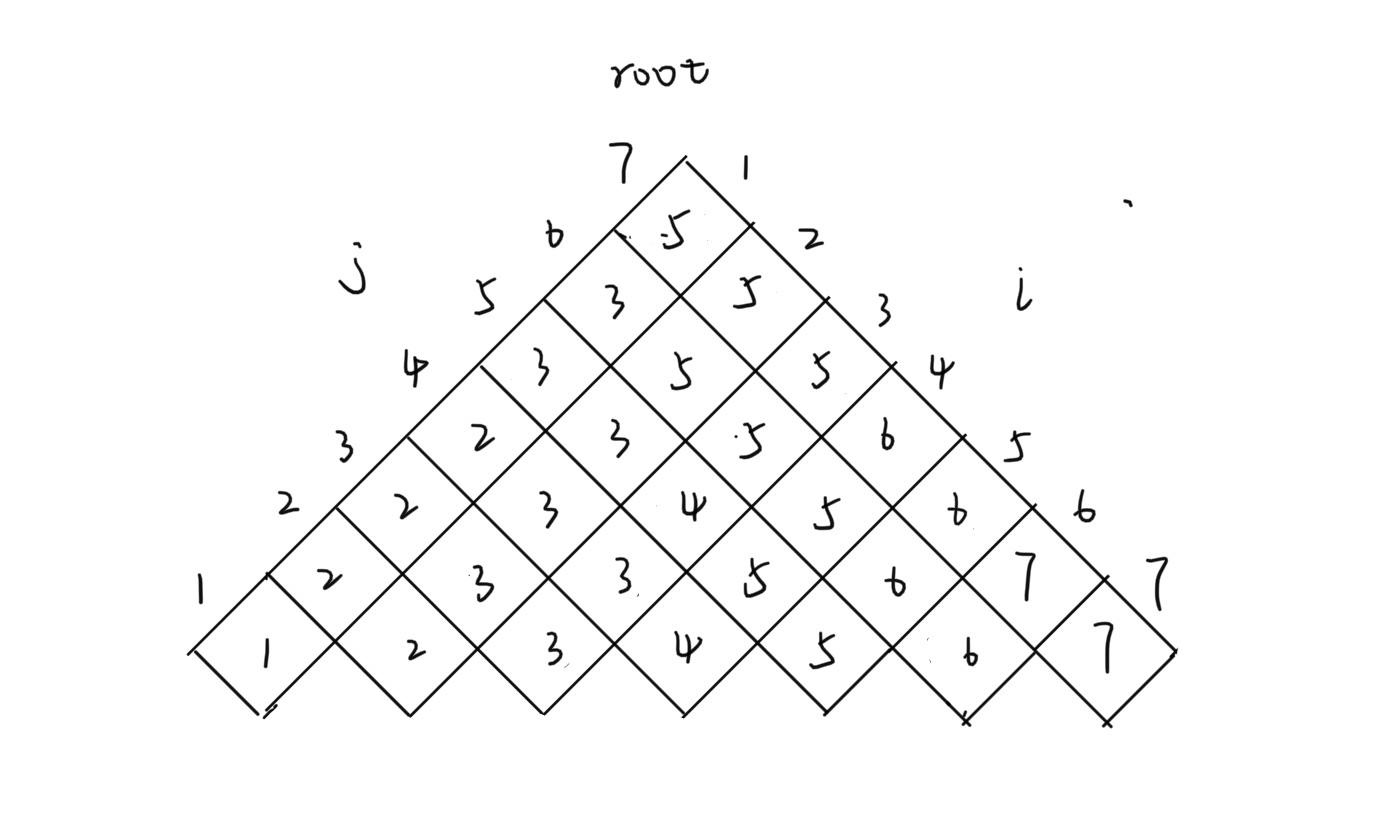
\includegraphics[scale = 0.2]{images/3_4.png}
		\end{minipage}
	\end{figure}
	\section{公司聚会}
	由于员工不能和其直接主管同时出席,同时为了使参会人数最大化,当一个员工出席时,对他的所有孙子节点为root的子树进行动态规划;若一个员工没有出席,那么对他的所有子节点进行动态规划。又由于关系树是采用的孩子兄弟表示法,变为如下策略:对所有出席对结点,对其右子树一直向右邀请出席(所有兄弟结点),而像左采用间隔邀请(孙结点)。
	\section{包含点列的闭区间}
	采用分治策略。每一次将n个点列分为$\lceil\frac{n}{2}\rceil$和$\lfloor\frac{n}{2}\rfloor$两部分,然后对这两部分分别递归调用。设区间左端点为$.lend$,右端点为$.rend$,则递推式为$all.lend = \min\{left.lend, right.lend\}, all.rend=\max\{left.rend, right.rend\}$。\par
	由分治策略的正确性可知此算法正确性显然
	\section{找零问题}
	算法:每一次都用最大面额的找零,直到余额为0为止。\par
	\begin{proof}
		若贪心算法选取的不是最优解,那么一定会发生以下几种情况之一:
		\begin{enumerate}
			\item 贪心选取了25美分的以及5美分和1美分的,但换为10美分是最优解:可能的子问题总额在25到35之间,只有30这部分可以用10美分找零,但$10+10+10\ (3)>25+5\ (2)$,故贪心为最优选择
			\item 贪心选取了10美分和1美分,但换为5美分为最优解:10为5的倍数,零钱数超过10的时候用一个10美分一定比用两个5美分要节省
		\end{enumerate}
		故贪心选取的是最优解
	\end{proof}

\end{document}
